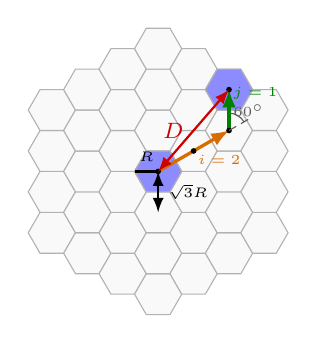
\begin{tikzpicture}[>=latex]
    \def\hexcell#1#2#3{\draw[fill=#3, draw=gray!60, shift={(#1,#2)}] (0:0.3) -- (60:0.3) -- (120:0.3) -- (180:0.3) -- (240:0.3) -- (300:0.3) -- cycle;}

    % Hexagonal grid with radius R = 0.3, axial axes at 30 deg (i) and 90 deg (j)
    \foreach \q in {-3,...,3} {
        \foreach \v in {-3,...,3} {
            \pgfmathtruncatemacro{\dist}{max(abs(\q),abs(\v),abs(\q+\v))}
            \ifnum\dist<4
                \pgfmathsetmacro{\cx}{0.45*\q}
                \pgfmathsetmacro{\cy}{0.5196*(\v+0.5*\q)}
                \hexcell{\cx}{\cy}{gray!5}
            \fi
        }
    }

    % Reference cell and nearest co-channel cell (i,j) = (2,1)
    \hexcell{0}{0}{blue!45}
    \hexcell{0.9}{1.0392}{blue!45}

    % Cell radius R and center spacing sqrt(3) R
    \draw[thick] (0,0) -- (180:0.3) node[midway, above, font=\tiny] {$R$};
    \draw[<->, thick] (0,0) -- (0,-0.5196) node[midway, right, font=\tiny] {$\sqrt{3}R$};

    % i steps along the first axis, then j steps after a 60 deg turn
    \draw[->, very thick, orange!85!black] (0,0) -- (0.9,0.5196)
        node[midway, below right, font=\tiny, text=orange!85!black, inner sep=1pt] {$i=2$};
    \draw[->, very thick, green!50!black] (0.9,0.5196) -- (0.9,1.0392)
        node[pos=0.9, right, font=\tiny, text=green!50!black, inner sep=1pt] {$j=1$};
    \foreach \x/\y in {0/0, 0.45/0.2598, 0.9/0.5196, 0.9/1.0392} {
        \filldraw (\x,\y) circle (0.8pt);
    }

    % 60 deg turn between the two axes (enclosed triangle angle is 120 deg)
    \draw[densely dashed, gray!70!black] (0.9,0.5196) -- ++(30:0.35);
    \draw[gray!70!black] (0.9,0.5196) ++(30:0.22) arc[start angle=30, end angle=90, radius=0.22];
    \node[font=\tiny, gray!70!black] at (1.15,0.77) {$60^\circ$};

    % Co-channel distance D
    \draw[<->, thick, red!80!black] (0,0) -- (0.9,1.0392)
        node[midway, left, font=\footnotesize, text=red!80!black] {$D$};
\end{tikzpicture}
